\chapter{\label{chap:state-of-the-art}State of the Art}
\section{Decentralized audio streaming services}
Multiple decentralized audio streaming services exist. Examples are Audius\footnote{\url{https://audius.co}}, Resonate\cite{lindner2018investing} and eMusic\footnote{\url{https://eMusic.com}}. All of these systems have in common that they save metadata and identifiers of audio files on a blockchain, and save the audio files in an off-chain database. All these off-chain databases are structured like IPFS\footnote{\url{https://ipfs.io/}} with a company-run centralized interface between the user interface and the database. For a system to be fully decentralized, this layer should be removed. These solutions are closed source. Moreover, they use their own cryptocurrency to pay their artists which is an unstable income.

\section{TrustChain-Superapp}
\label{sec:sote-trustchain}
The TrustChain superapp~\citep{mattskala2020} is a framework for implementing mobile Android decentralized applications. It allows for storing append-only immutable data on TrustChain~\citep{otte2020trustchain} and spreading this data in a phone-to-phone serverless network. It follows the concept of super apps~\citep{kpmg2019superapps}, meaning that it contains many mini-apps which use the same networking interface. The Superapp is an Android app as seen in fig. \ref{fig:trustchain-superapp}. Its mini-apps implement decentralized democratic voting and has bitcoin payment integration, among other features.

\begin{figure}
    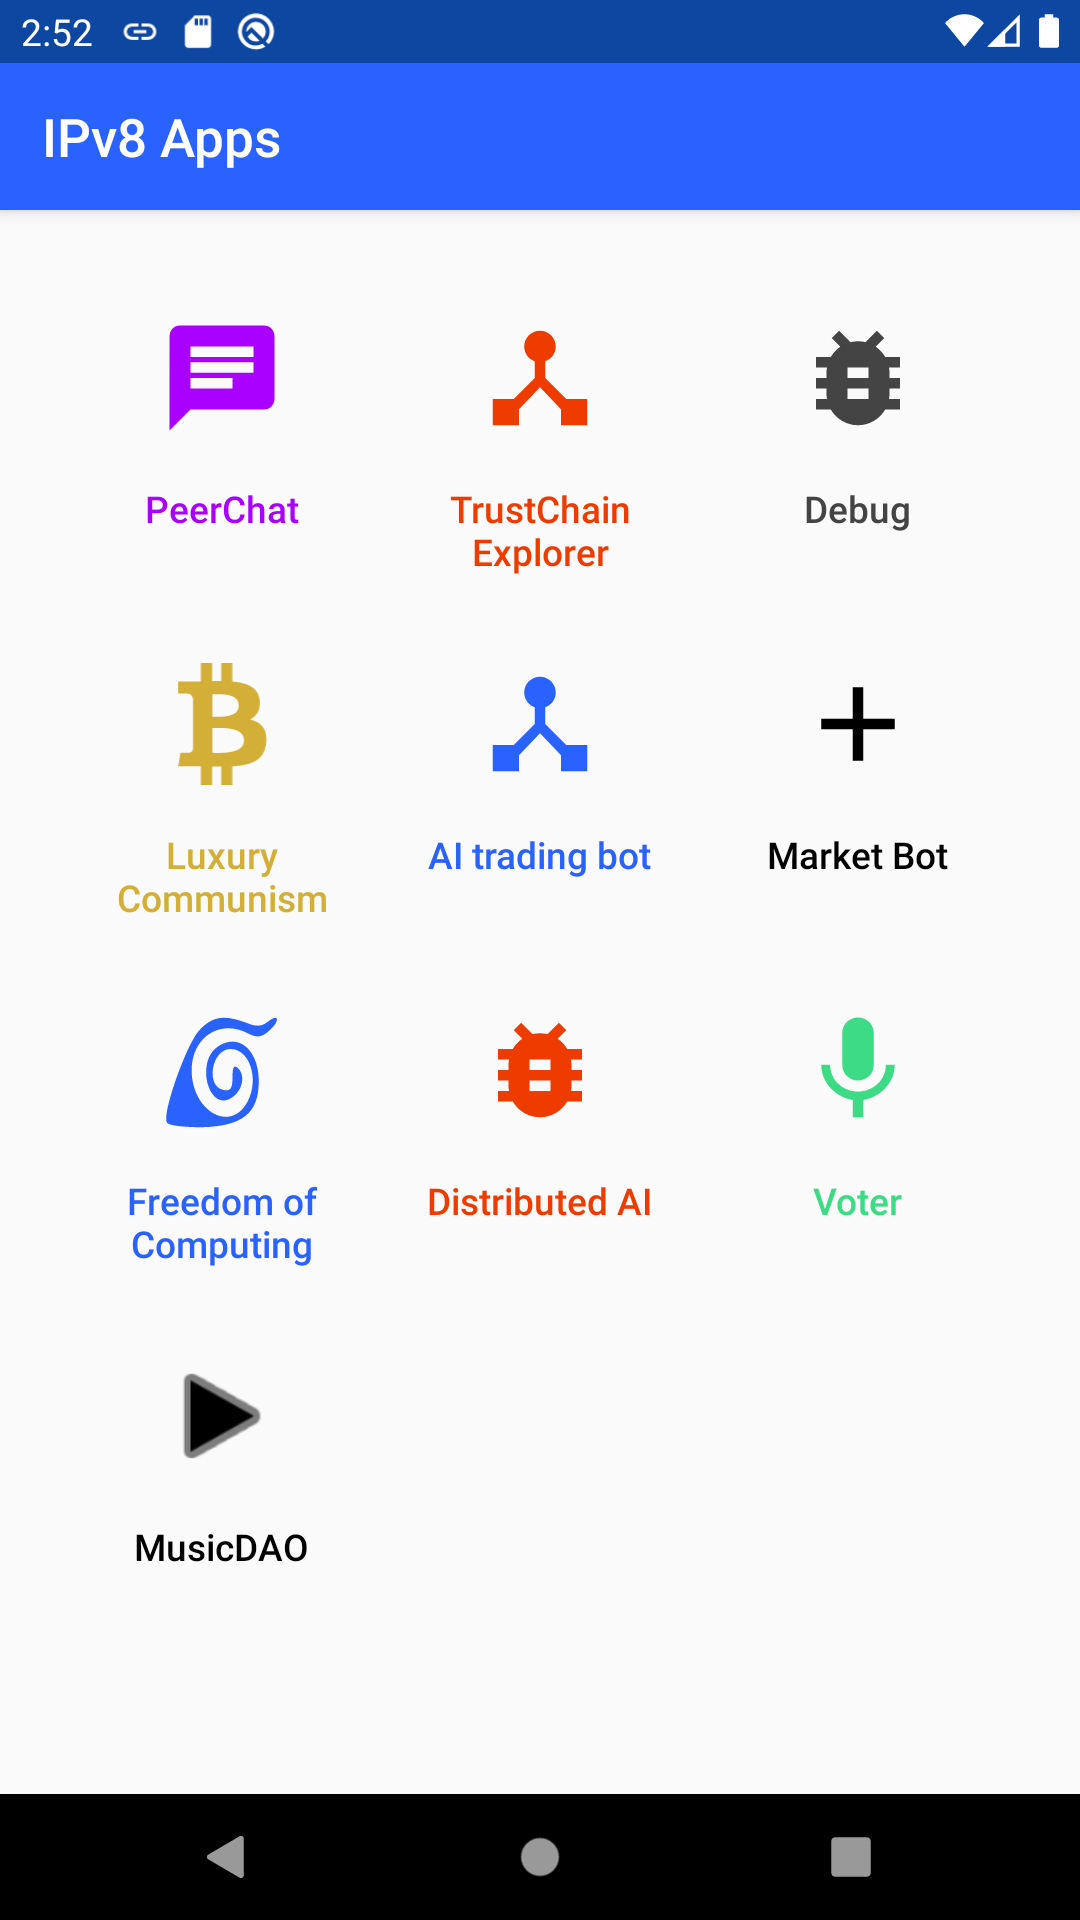
\includegraphics[width=0.3\textwidth]{implementation/screenshot-superapp.png}
    \caption{Trustchain-Superapp overview}
    \label{fig:trustchain-superapp}
\end{figure}

\section{Tribler and bandwidth tokens}
Tribler is a peer-to-peer system to share, download and stream multimedia. It has implementations for desktop environments and an Android prototype. It makes use of BitTorrent for file transfer and adds anonymization techniques on top of it. In addition, it makes use of its bandwidth tokens: an incentive system to increase cooperation between users, in order to achieve high availability of downloads. In essence, it subtracts tokens for downloading content from peers and rewards tokens for helping peers. An overview of the Tribler desktop interface can be seen in fig. \ref{fig:tribler}.

\begin{figure}
    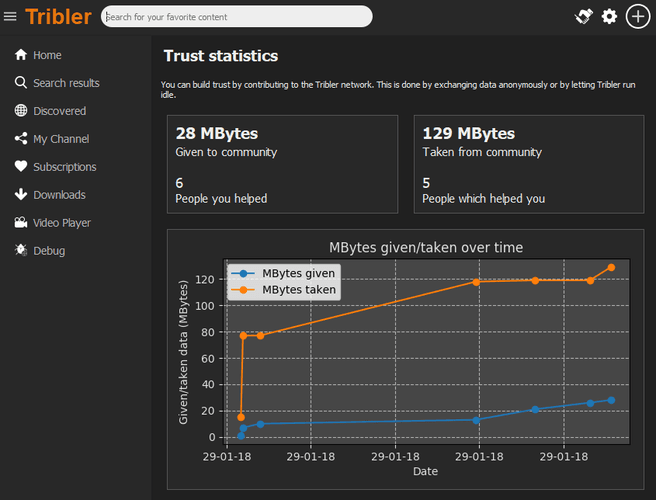
\includegraphics[width=0.7\textwidth]{related-work/tribler7.3.0.png}
    \caption{Tribler desktop interface, showing the bandwidth incentive system overview}
    \label{fig:tribler}
\end{figure}

\section{Decentralized content delivery networks}
Decentralized content delivery networks are being investigated by multiple systems such as VideoCoin\footnote{\url{www.videocoin.io}} and DCDN\footnote{\url{https://www.dcdn.com/}}. Most of these start-ups use blockchain technology and their own-released cryptocurrency as a token to pay nodes that serve the content. This means that the incentive for running a node depends on the value of those cryptocurrencies, so this is an unstable situation for workers. 

A fully decentralized audio streaming service requires sharing and streaming audio files over a network of nodes in which any participant can start and run a node. An example of such network is BitTorrent. The challenge with BitTorrent acting as a streaming service is that the requirement from the user perspective is to have low latency for streaming and buffering media files. For each file, the peer discovery algorithm is run, which is a slow-start algorithm. It also relies on having enough seeders per file available.

Torrent files contain a list of chunks, which represent the different parts of the related file. These chunks are called torrent pieces. Flawless streaming of media files over BitTorrent requires a smart algorithm to predict what file is requested next, and what torrent pieces should be loaded. BitTorrent relies on trackers to perform peer discovery. However, trackers are a central point of failure. To make the system more decentralized, a solution using independent trackers and a gossip protocol\cite{dan2011efficient} can be used. 

\section{Incentives for file spreading}
In a DAO, the party responsible for hosting and spreading of files is not well-defined. To tackle the tragedy of the commons, entities should be incentivised just enough for the system to be sustainable and usable, but no more. An example incentive system is bandwidth tokens~\citep{de2018blockchain}.

% TODO READ/DISCUSS FOLLOWING RELATED WORK:
% https://github.com/javto/Tribler-streaming
% Decentralized Media Streaming on Android using Tribler